%% Lab Report for EEET2493_labreport_template.tex

%Next line necessary for no xelatex errors 
\RequirePackage[OT1]{fontenc} 
\documentclass[journal]{IEEEtran}

\usepackage{mathtools}

%font packages
\usepackage[utf8]{inputenc}

% *** CITATION PACKAGES ***
\usepackage[style=ieee]{biblatex} 
\bibliography{example_bib.bib}    %your file created using JabRef

% *** MATH PACKAGES ***
\usepackage{amsmath}

% *** PDF, URL AND HYPERLINK PACKAGES ***
\usepackage{url}
% correct bad hyphenation here
\hyphenation{op-tical net-works semi-conduc-tor}
\usepackage{graphicx}  %needed to include png, eps figures
\graphicspath{{./images/}}
\usepackage{float}  % used to fix location of images i.e.\begin{figure}[H]
\usepackage{array}
\usepackage{tabularx}

\begin{document}

% paper title
\title{RF Lab Module \#1 - Scalar Measurements} %\\ \small{Title of the session (you can be creative highlighting your findings)}}

% author names 
\author{ Stephen Campbell } 
    
        
% The report headers
\markboth{EE/CE 4202 Electrical and Computer Engineering Laboratory in Circuits. Lab \#1, \today }%do not delete next lines
{Shell \MakeLowercase{\textit{et al.}}: Bare Demo of IEEEtran.cls for IEEE Journals}

% make the title area
\maketitle

% As a general rule, do not put math, special symbols or citations
% in the abstract or keywords.
\begin{abstract}
In this lab, the speed of light was measured with method utilizing household materials and tools.
Next, familiarity with scalar radio frequency power measurements was gained. Several cables, attenuators,
and filters were measured to affirm their specification.
\end{abstract}

% \begin{IEEEkeywords} %indicate keywords that cover the topic
% keywords, temperature, xxxx equation, etc.
% \end{IEEEkeywords}

\section{Introduction}
% Here we have the typical use of a "W" for an initial drop letter
% and "RITE" in caps to complete the first word.
% You must have at least 2 lines in the paragraph with the drop letter
% (should never be an issue)

\IEEEPARstart{T}{o} gain understanding of radio frequency (R.F.) power measurements and standing
waves, several measurements were conducted and analyzed. First, the speed of light was measured by utilizing 
a microwave's ability to generate a standing wave with a particular frequency. To measure 
different R.F. components, a  R.F. signal generator, power sensor, and power meter were utilized.
With a proper introduction and basic understanding of these tools, several components were measured
including cables, attenuators, and a filter.


\section{Speed of Light Experiment}

\subsection{Procedure}

To measure the speed of light using a microwave, the rotating plate was removed
from the appliance. Sliced cheese was the placed onto a paper plate inside of
the microwave. After 15 seconds in the microwave, the cheese platter was
examined. There were regions of soft, melted cheese and hard, cold cheese.
Because the microwave forms standing waves during operation, it is implied that
the hot spots correspond to the standing waves antinodes. The distance between
adjacent antinodes corresponds to half wavelengths of the standing wave. With the half wavelengths known,
the full wavelength can be determined. The measurements taken are recorded in Table \ref{table:speed}.

\begin{table}[htbp]
    \centering
        \caption{Observations and measurements for calculating the speed of light  \label{table:speed}}
        \begin{tabular}{|c|c|}
            \hline
            \textbf{Measurement Type}         & \textbf{Value} \\ \hline
            Frequency of microwave operation & 2.45 GHz       \\ \hline
            Distance between hotspots         & 5.75 cm        \\ \hline
        \end{tabular}
\end{table}

\begin{align*}
\frac{\lambda }{2} & =5.75\times 10^{-2}\text{m}\\
\lambda  & =11.5\times 10^{-2}\text{m}\\
f & =2.45\times 10^{9}\text{Hz}\\
 & \\
c_{\text{measured}} & =\lambda f\\
c_{\text{measured}} & =\left( 11.5\times 10^{-2}\right)\left( 2.45\times 10^{9}\right)\\
c_{\text{measured}} & =2.8175\times 10^{8} \\
\end{align*}
\begin{align*}
\%\ \text{error} & =\frac{|c-c_{\text{measured}}{} |}{c}\\
\%\ \text{error} & =\frac{|2.99\times 10^{8} -2.8175\times 10^{8} |}{2.99\times 10^{8}} \cdot 100\%\\
\%\ \text{error} & =0.05\ \cdot 100\%\\
\%\ \text{error} & =5\%
\end{align*}


\subsection{Analysis}

The accuracy of the speed of light measurement was dependent on several factors.
The factors likely caused the drift between the measured speed of light and the
theoretical speed of light. These factors include, but are not limited to:
\begin{itemize}
    \item Tolerance of the generated frequency of the microwave 
    \item Measurement error using the ruler
    \item Operator error related to the ambiguity of the exact location of the antinodes
\end{itemize}
With these factors in mind, the percent error of 5\% is entirely reasonable. Some
problems include the ambiguity with the exact location of the antinodes. It
seemed as if the antinodes occurred at the seams of the cheese slices. A
solution to fix this problem would be to procure a larger cheese sheet and to
leave the microwave on for longer. With these 2 modifications, the ambiguity of
the antinode location would be minimized. Another problem is the limited sample
size. This subjects the measured value to random errors. By collecting more
samples, one could gain more confidence in the measurements.

\section{Power Meter Experiment}

\subsection{Attenuators}
The measured power of the signal generator's 2GHz 0 dBm signal (2.c) was -0.12
dBm. For a 2 GHz frequency, several measurements and calculations were made for
different attenuators as shown in Table \ref{table:attenuators}.

\begin{table*}[htbp]
    \newcommand{\ct}{\centering\arraybackslash}
    \centering
    \caption{Attenuator Scalar power measurements and calculations performed during the lab session 
                \label{table:attenuators}
            }
    \begin{tabularx}{0.8\textwidth}{*{6}{|>{\ct}X}|}
        \hline
        \textbf{Medium}     & \textbf{Absolute Power (dBm)} & \textbf{Absolute Power (mW)} & \textbf{Insertion Loss (dB) at 2GHz} & \textbf{Insertion Loss Difference Absolute (dB)} & \textbf{Insertion Loss Difference Percentage} \\ \hline
        RF Cable            & -0.12                         & 0.972747                     & -0.12                                & N/A                                              & N/A                                           \\ \hline
        3dB SMA attenuator  & -3.8                          & 0.416869                     & -3.8                                 & -0.8                                             & 26.667                                        \\ \hline
        10dB SMA attenuator & -10.28                        & 0.0937562                    & -10.28                               & -0.28                                            & 2.8                                           \\ \hline
        20dB SMA attenuator & -20.17                        & 0.00961612                   & -20.17                               & -0.17                                            & 0.85                                          \\ \hline
    \end{tabularx}
\end{table*}

\subsection{Filter}

A R.F. bandpass filter attenuation was measured at frequencies well below its
nominal pass band through frequencies above the pass band.  These measurements
recorded and appear in Table \ref{table:filter} and Fig. \ref{fig:filter}.

\begin{table}[htbp]
    \centering
    \caption{Band pass filter scalar power measurements performed over frequency range
    \label{table:filter}
    }
    \begin{tabular}{|c|c|}
        \hline
        \textbf{Frequency (GHz)} & \textbf{Absolute Power (dBm)} \\ \hline
        1                        & -36.00                        \\ \hline
        1.25                     & -34.42                        \\ \hline
        1.5                      & -40                           \\ \hline
        1.75                     & -28                           \\ \hline
        2                        & -9.32                         \\ \hline
        2.25                     & -1.86                         \\ \hline
        2.5                      & -2.07                         \\ \hline
        2.75                     & -6.94                         \\ \hline
        3                        & -12.99                        \\ \hline
        3.25                     & -12.6                         \\ \hline
        3.5                      & -23.47                        \\ \hline
        3.75                     & -27.10                        \\ \hline
        4                        & -32.01                        \\ \hline
    \end{tabular}
    
\end{table}

% %you can use a table generator from here: https://www.tablesgenerator.com/#

% Use your word processor to make “real tables” (i.e., boxed in, etc.). Center all tables and include a heading and caption with the appropriate table number below each table. For example, “Table 1: Temperature measurements performed for session 1.” 

% Figures must be centered, and the figure number and caption is centered beneath the
% figure. For example, “Figure~\ref{fig:ecg}”. 

\begin{figure}[htbp]
    \centering
        \caption{Filter Power Transmission
        \label{fig:filter}
        }
    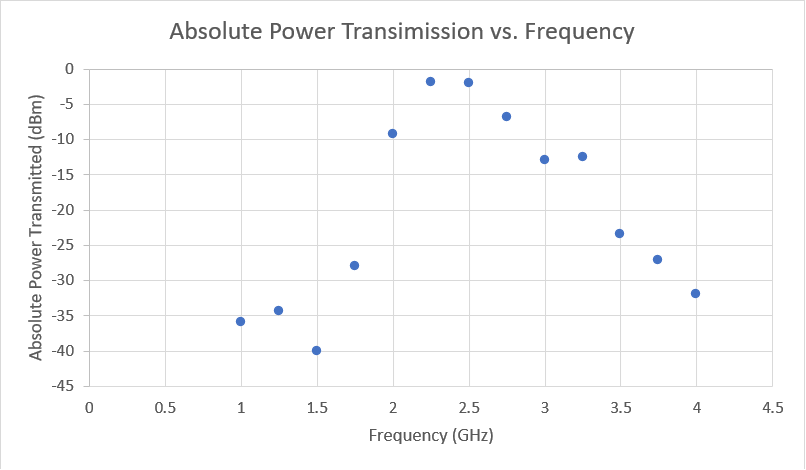
\includegraphics[width=0.4\textwidth]{filter_transmission.png}
\end{figure}


\section{Conclusion}
\subsection{Question to Consider}

\textbf{From what you learned in lab today why do microwave oven manufacturers
almost always include a rotating platform?}

The rotating platform reduces the uneven heating that the microwave produces.
From the food’s perspective, the nodes/antinodes are constantly changing
positions so the food cooks more evenly than it would be otherwise.    

\appendices
% \section{Pre-Lab}
% List any extra evidence such as photos of the session, that may help you support your claims.
% You can include all hand calculations, extra graphs and plots, simulation results, etc. 

\section{Extra Photos}

\begin{figure}[htbp]
    \centering
    \caption{Cheese slices that were measured to determine the speed of light
        \label{fig:cheese}
    }
    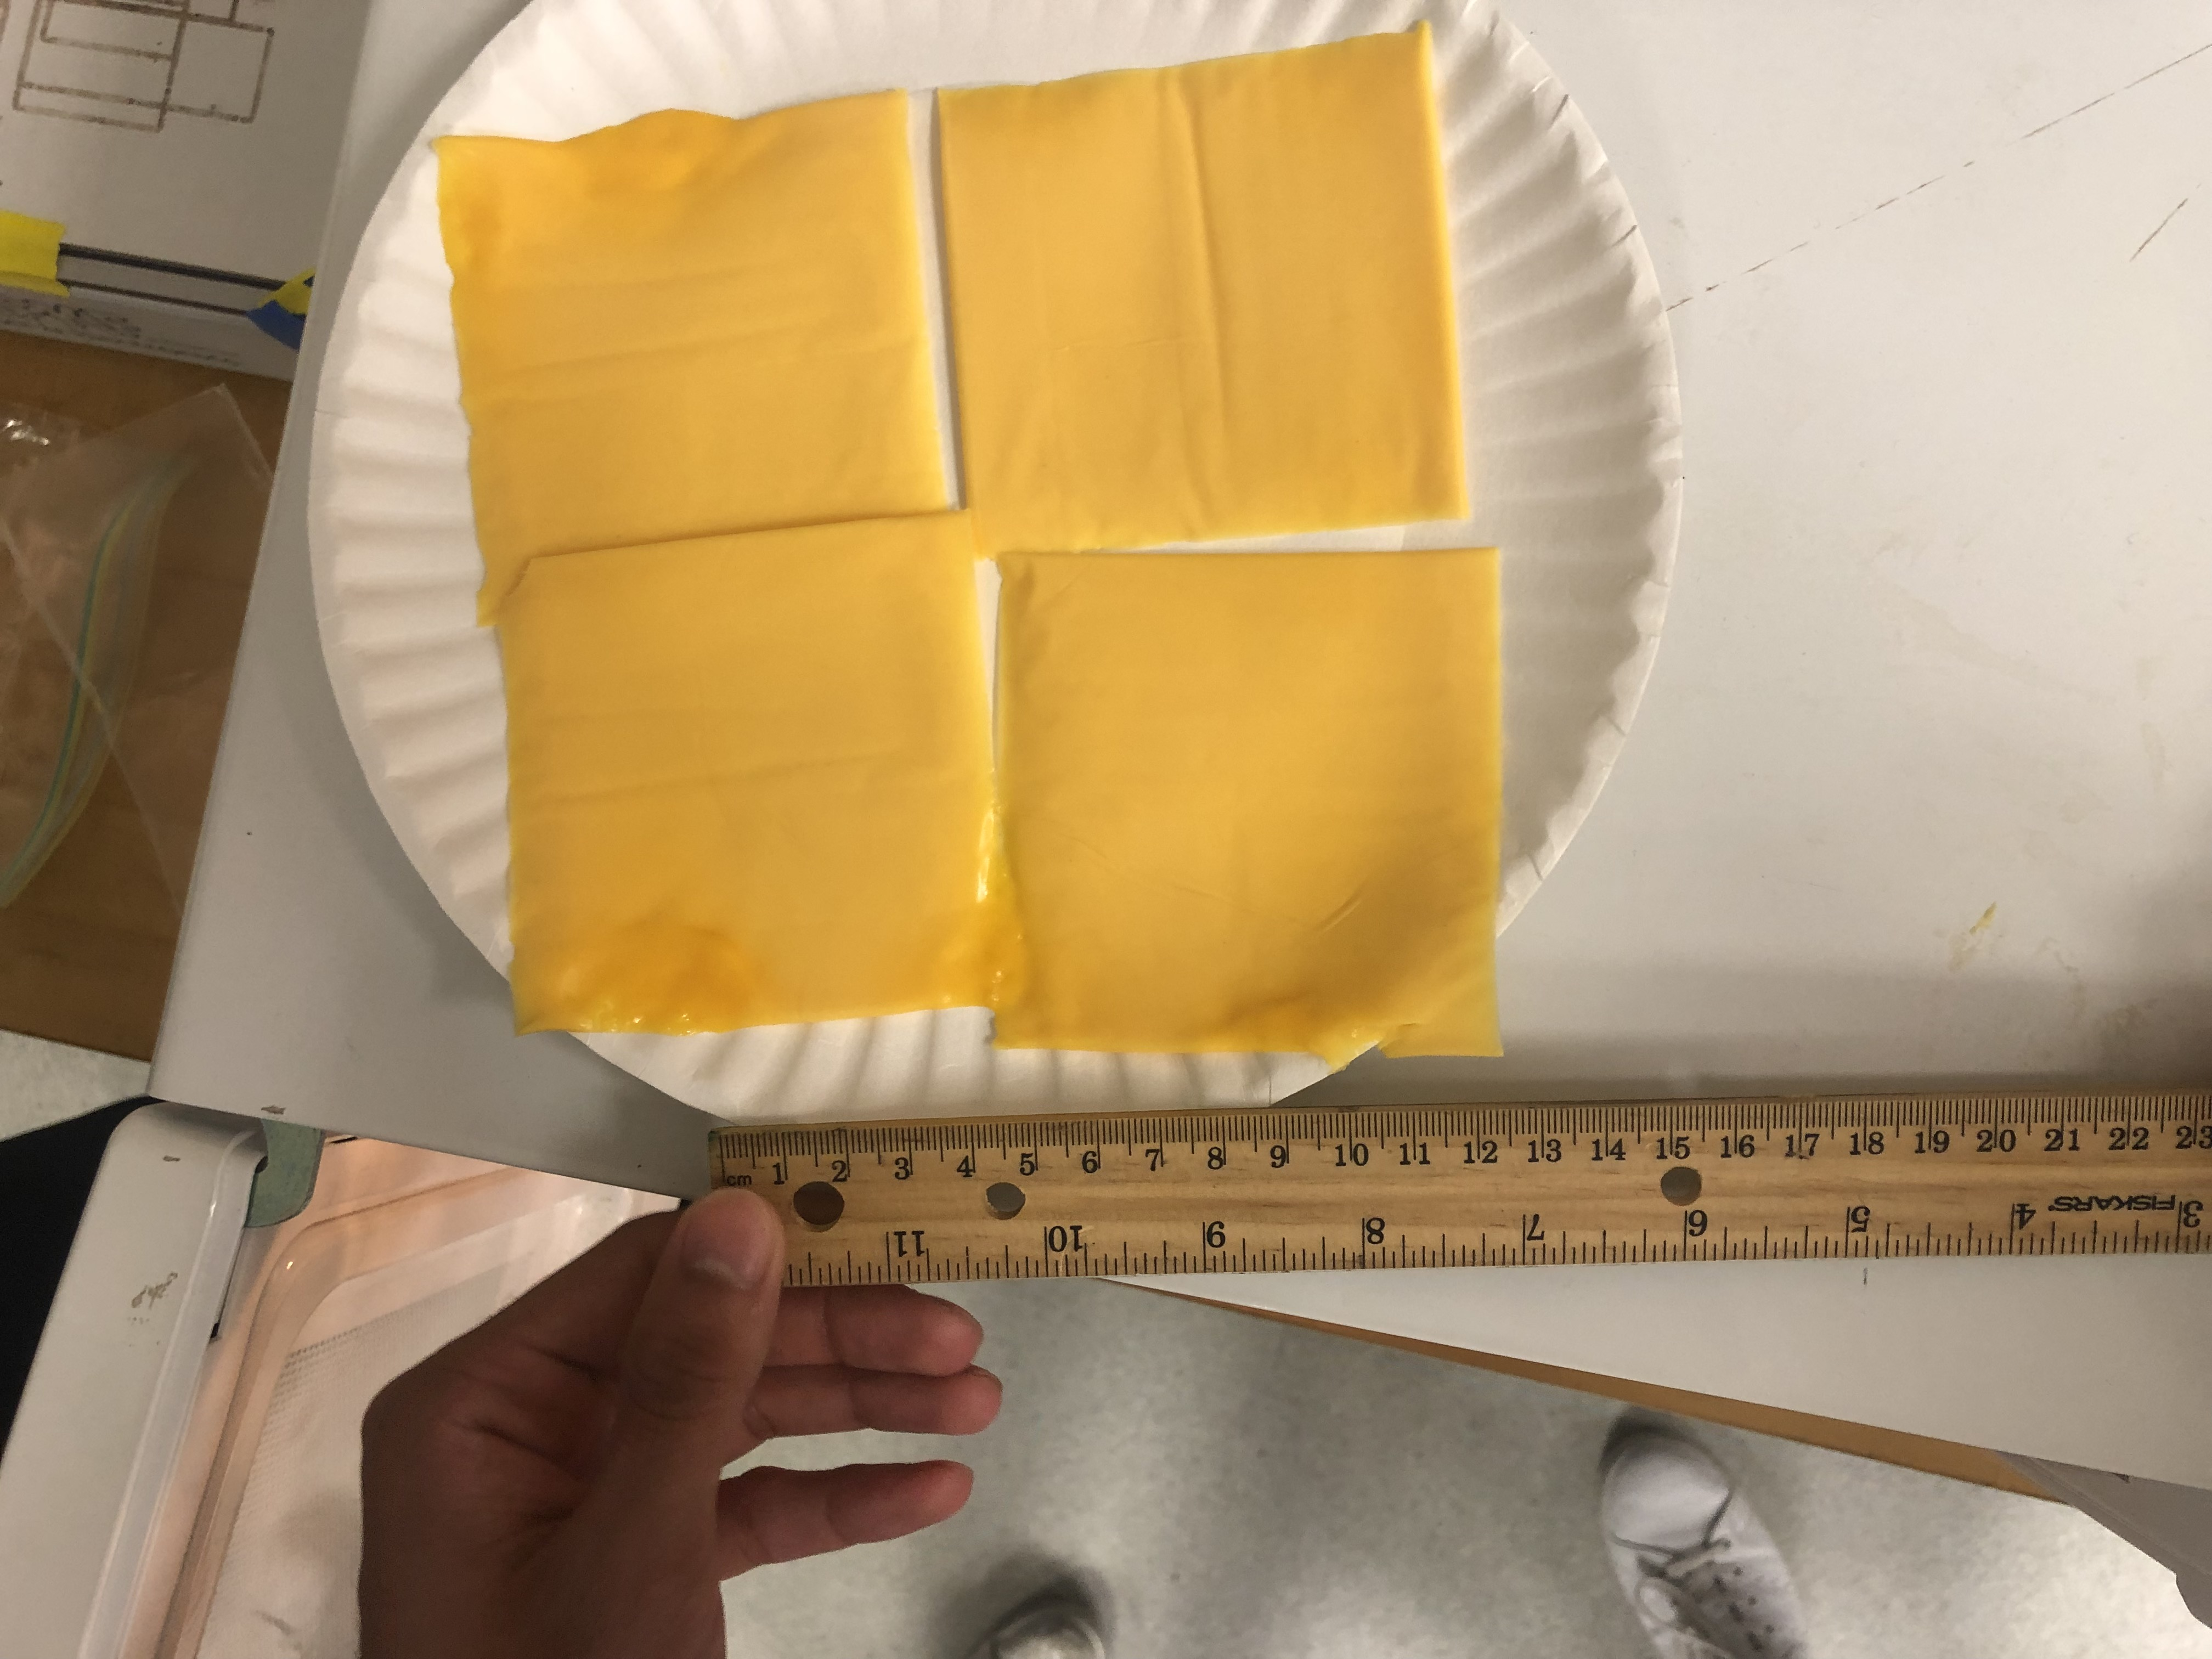
\includegraphics[width=0.3\textwidth]{cheese.jpg}
\end{figure}



% use section* for acknowledgment
%\section*{Acknowledgment}
%The authors would like to thank...



% references section

% can use a bibliography generated by BibTeX as a .bbl file
% BibTeX documentation can be easily obtained at:
% http://mirror.ctan.org/biblio/bibtex/contrib/doc/
% The IEEEtran BibTeX style support page is at:
% http://www.michaelshell.org/tex/ieeetran/bibtex/
%\bibliographystyle{IEEEtran}
% argument is your BibTeX string definitions and bibliography database(s)
%\bibliography{IEEEabrv,../bib/paper}
%
% <OR> manually copy in the resultant .bbl file
% set second argument of \begin to the number of references
% (used to reserve space for the reference number labels box)

%use following command to generate the list of cited references

\end{document}


